\documentclass[russian,a4paper,12pt]{scrartcl}
\usepackage{babel}
\usepackage[utf8]{inputenc}
\usepackage[left=3cm,right=1cm,top=1cm,bottom=1cm]{geometry}
\usepackage{misccorr}
\usepackage{amsmath}
\usepackage{minted}
\usepackage{graphicx}
\usepackage{xcolor}
\usepackage{hyperref}
 % Цвета для гиперссылок
\definecolor{linkcolor}{HTML}{799B03} % цвет ссылок
\definecolor{urlcolor}{HTML}{799B03} % цвет гиперссылок
\hypersetup{pdfstartview=FitH,  linkcolor=blue,urlcolor=blue, colorlinks=true}

\begin{document}
	\begin{center}
	
		\large{МИНИСТЕРСТВО ОБРАЗОВАНИЯ И НАУКИ\\ РОССИЙСКОЙ ВЕДЕРАЦИИ} \par
		\bf\MakeUppercase{федеральное государственное автономное образовательное учреждение высшего образования} \par
		\textit{<<Санкт-Петербургский Государственный университет 
		Аэрокосмического Приборостроения>>} \par
	
	\vspace{10mm}
		
		\MakeUppercase{Кафедра №14} \par 
		
	\vspace{20mm}
	\begin{flushleft}
		{ОТЧЕТ}\par
		{ЗАЩИЩЕН С ОЦЕНКОЙ}\par
		{ПРЕПОДАВАТЕЛЬ}\par
	\end{flushleft}
	\begin{flushleft}
			\underset{\text{должность}}{\underline{\hspace{1cm}\text{асс.}\hspace{1cm}}}\quad\underset{\text{подпись, дата}}{\underline{\hspace{4cm}}}\quad\underset{\text{инициалы, фамилия}}{\underline{\hspace{1cm}\text{П.С. Санкин}\hspace{1cm}}}
	\end{flushleft}
	\vspace{10mm}

		 \textbf{ОТЧЕТ О ЛАБОРАТОРНОЙ РАБОТЕ №1}\par\vspace{5mm}{РАСТРОВЫЕ ИЗОБРАЖЕНИЯ}\par{По курсу: <<Основы мультимедия технологий>>.} \par
		
	\vspace{40mm}

	\begin{flushleft}
		{РАБОТУ ВЫПОЛНИЛ}\par
		\begin{flushleft}
			СТУДЕНТ ГРУППЫ \underline{1441} \quad\underset{\text{подпись, дата}}{\underline{\hspace{4cm}}}\quad
			\underset{\text{инициалы, фамилия}}{\underline{\hspace{0,5cm}\text{А.А. Протасов}\hspace{0,5cm}}}
		\end{flushleft}
	\end{flushleft}

	\vspace{50mm}
	
		{Санкт-Петербург\\ 2016}
	\thispagestyle{empty}
	\newpage
	
	\end{center}

	\begin{flushleft}
	\setcounter{page}{2}
		\section{Цель работы}
			Получение практических навыков работы с растровыми изображениями, научиться проводить простейшую обработку растровых изображений.
		\section{Постановка задачи}
			Для графических файлов в формате BMP/PNG написать программу, выполняющую заданное графическое преобразование с выводом результата. Файлы изображений для программы создать самостоятельно.
		\section{Задание}
			Залить все изображение черным.
		\section{Краткие теоритические сведения}
			Существует множество форматов для хранения растровых изображений. Самые популярные из них PNG и BMP. BMP - формат хранения растровых изображений, разработанный компанией Microsoft. Файлы формата BMP могут иметь расширения .bmp, .dib и .rle. PNG - растровый формат хранения графической информации, использующий сжатие без потерь по алгоритму Deflate.
		\section{Описание метода реализвции}
			Используя среду разработки Qt Creator. Файл с картинкой был заранне выбран и самим Qt при инициализации был преобразован в 32-бита. В листинге предоставлен код прогрвммы, которая заливает все изображение черным цветом.
		\newpage
		\section{Листинги}
		\usemintedstyle{autumn}
			\begin{minted}[
				frame=lines,
				framesep=2mm,
				baselinestretch=1.2,
				fontsize=\footnotesize,
				linenos
				]{cpp} 

#include<QApplication>
#include<QWidget>
#include<QHBoxLayout>
#include<QLabel>
#include<iostream>

int main(int argc, char *argv[])
{
    QApplication app(argc, argv);
    QImage       img("/home/toshiki/files/1280.png");
    QWidget      wgt;
    QHBoxLayout* phbx = new QHBoxLayout;
    QLabel*      plbl = new QLabel;

    phbx->setMargin(0);
    phbx->setSpacing(0);
    plbl->setPixmap(QPixmap::fromImage(img.scaled(img.width()/2,
    	img.height()/2,Qt::KeepAspectRatio)));
    phbx->addWidget(plbl);
    wgt.setLayout(phbx);

    qint32      height  = img.height();
    qint32      width   = img.width();
    for(qint32 y = 0; y < height; ++y){
        QRgb* tempLine = reinterpret_cast<QRgb*>(img.scanLine(y));
        for(qint32 x = 0; x < width; ++x){
            int alpha   = qAlpha(*tempLine);
            *tempLine++ = qRgba(0, 0, 0, alpha);
        }
    }

    QLabel*     plbl2 = new QLabel;
    plbl2->setPixmap(QPixmap::fromImage(img.scaled(img.width()/2,
    	img.height()/2,Qt::KeepAspectRatio)));
    phbx->addWidget(plbl2);
    wgt.setLayout(phbx);

    wgt.show();

    return app.exec();
}

			\end{minted}
		\section{Примеры работы программы}
			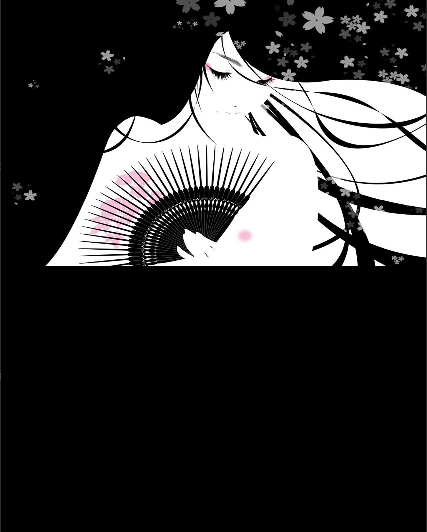
\includegraphics[scale=0.5]{Screenshot1}
		\section{Выводы}
			Получил практические навыки работы с растровыми изображениями в среде разработки Qt Creator. Научился проводить простейшую обработку растровых изображений.
	\newpage
	\begin{thebibliography}{9}
		\bibitem{Schlee-2015}Шлее М. Qt 5.3. Профессиональное программирование на C++ \newblock --- Санкт-Петербург:
		Изд.  БХВ-Петербург, 2015. 928~с.
		\bibitem{Link} \href{http://doc.qt.io/qt-5/reference-overview.html}{\underline{http://doc.qt.io/qt-5/reference-overview.html}}
		\bibitem{Guide}Методические указания по курсу: ОСНОВЫ МУЛЬТИМЕДИАТЕХНОЛОГИЙ
	\end{thebibliography}
\end{document}